% Version 0.3
\section{Version 0.3}

In the third version the goal was to learn if people actually want to use the application to keep track of books they borrow or have lent to others. From the previous versions the indication says that they do, but according to Lean Startup it is not possible to know if it is correct until it can be proven scientifically with data measured. As in the earlier versions this version contains two iteration, one for with paper prototypes and one with the implemented application.
\subsection{Assumption and questions}
The assumption to be confirmed for this iteration was
“Users want to borrow books and be able to keep track of who has borrowed the book and who they have borrowed the book from”.

Questions needed to confirm this assumption: 
\begin{enumerate}
\item Is there a market for borrowing books among the users?
\item Do the users tend to have trouble remembering who they borrowed a book from?
\item Is it a problem for the users to remember what books are borrowed?
\end{enumerate}

\subsection{Planning and design}
To confirm the assumption selected in this version, the team had to learn about the users book habits. How often the users borrow books and how often there is a problem keeping track of a book, are essential issues to learn how the users will adapt to the application. In obtaining these answers, the team planned to do a usability test with questions for the students and to ask the employees at Netlight. 

Indeed the most vital information about the users is collected by measuring the use of the application, but because of the application’s small user base those numbers may also be an unrepresentative result. One of the reasons the application has not managed to get the desired number of users is that the application is not satisfying to be a product, or minimal viable product to Netlight. Because of this the customer representative will deploy the application to Netlight when certain functionality is implemented and until then the team should follow the \gls{LSU} with numbers from prototypes and surveys, and of course the small amount of data retrieved from users of the application. 

In developing a paper prototype the team discussed the different possibilities of how to represent the borrowed and lent books, in addition to the representation of a borrow-functionality. The different possibilities were drawn on the whiteboard in accordance to Lean UX and eventually the team agreed upon a design. Because of the new feature of showing what books a users has lent, the shelf view was switched from alternative 1 to alternative 2 shown in figure \ref{fig:design-alternatives-v2}, but with three lists instead of two. The new paper prototype created is illustrated in figure \ref{fig:prototype-v3} where each view was a cut out in phone size when presented to the users. 

From the discussion of functionality needed in this version to learn about the assumption, five user stories were selected as requirements. These are shown in \ref{user-stories-v3}. When conducting the usability test these stories were used as basis for the tasks the participants had to complete. 

\begin{figure}
\centering
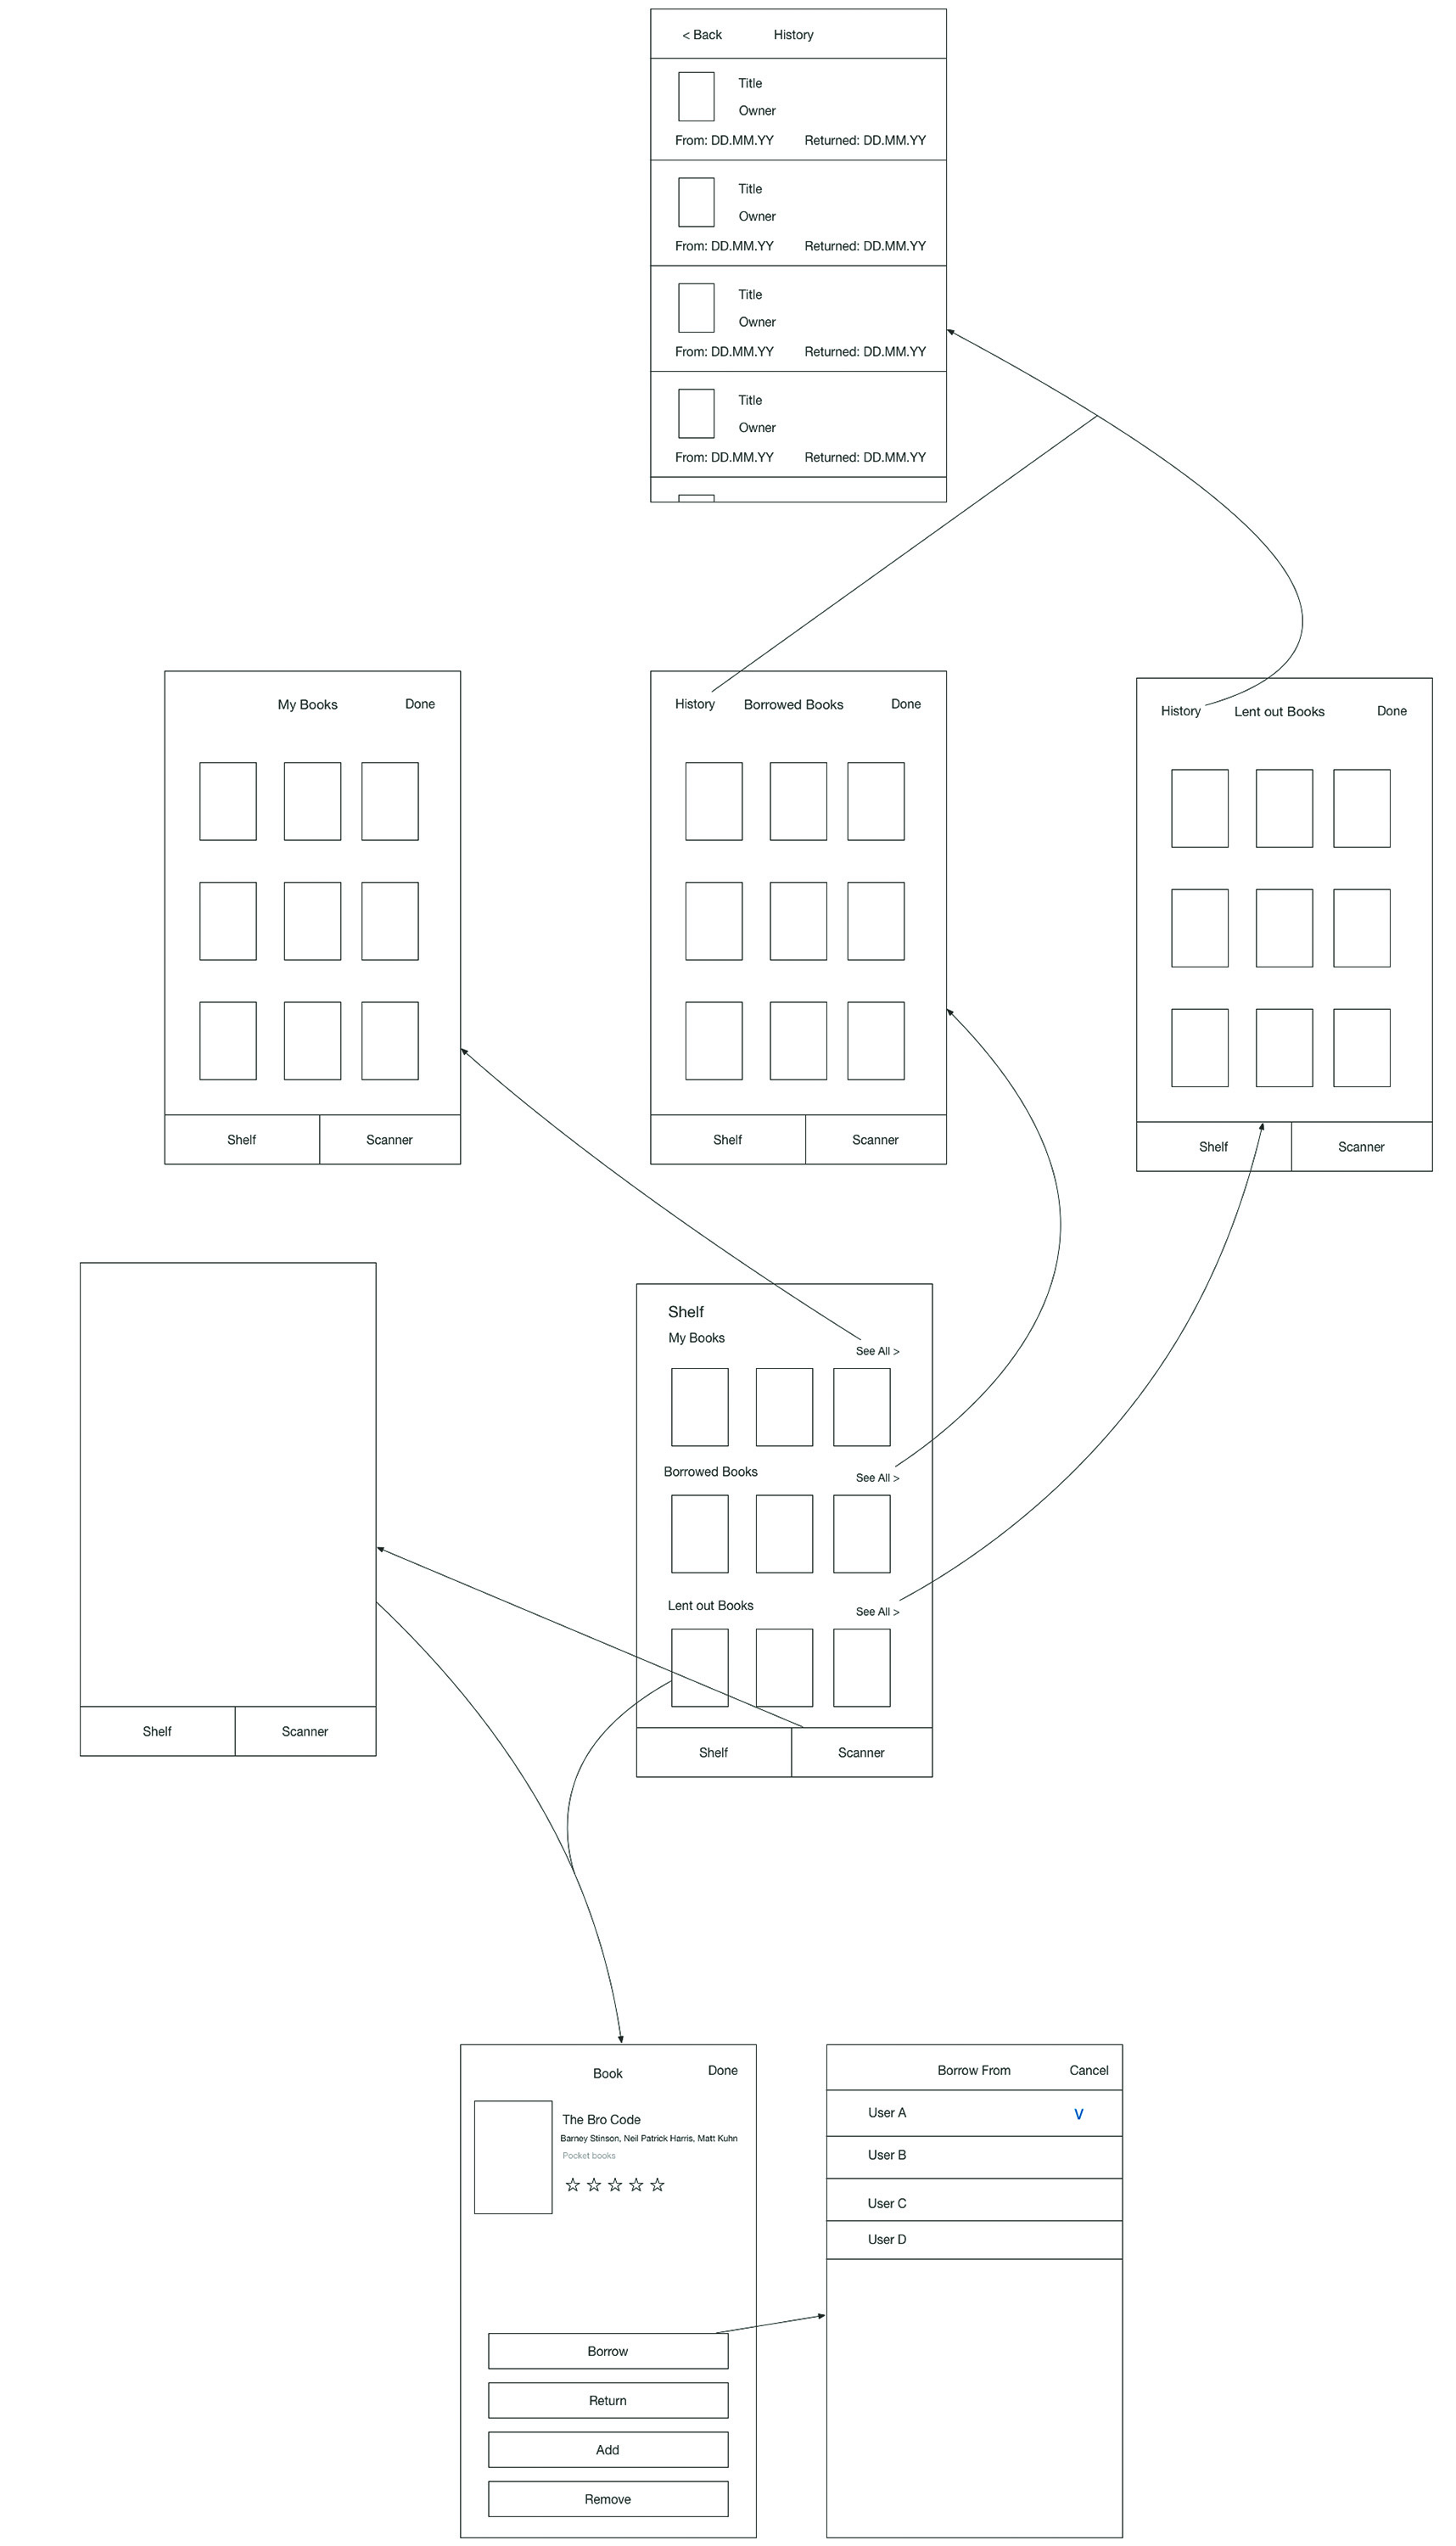
\includegraphics[height=20cm]{figs/v03/prototypesv3.jpg}
\caption{Relationship between views of paper prototype for CrowdShelf version 0.3}

\label{fig:prototype-v3}
\end{figure}

The usability test started with explaining the product, then the users were given the start screen and asked to complete the following tasks:
\begin{enumerate}
\item Borrow a book.
\item See a list of all books you own, but are lent out.
\item See a list of all books you have that are not yours.
\item Return a book you have borrowed.
\end{enumerate}

After the test was completed the application had a design of the functionality and the team was ready to implement the user stories in the application.




\subsection{User stories}
\label{user-stories-v3}
This section shows the user stories selected as requirements version 0.3. The stories are selected based on the assumption thought to be the most relevant to test the features of the product. 

\begin{enumerate}
  \item As a user I want to borrow a book from another member  
  \item As a user I want to return a book that i have borrowed
  \item As a user I want to see the owner and holder of all copies of a book
  \item As a user I want to see a list of all the books I'm currently borrowing
  \item As a user I want to see a list of all the books I'm lending to others
\end{enumerate}



\subsection{Development}
Developing the new features of this version was easier than the earlier version because the development teams were starting to get a better take on the implementation. This section explains in detail what was created during this version iteration in the three different sub teams.

\subsubsection{Android}
\begin{description}
    \item[Features] \hfill\\
The first task the Android team focused on for this version was the ability to borrow a book from another user, and register this for both users involved. To be able to do this, the application needed to show which users who owned a specific book, and then be able to select a user to borrow this book from. To implement this a group were created containing all the Android users of the application. This was done because the team had future releases in mind, which probably would include the possibility to create groups of users. Therefore instead of implementing the possibility of listing all users, which would not be used later at any time, the team implemented a solution were all users where in a single group, and then listing the members of this group, a feature that was probably going to get used in future releases. 

Then, when a user wanted to borrow a book, the group was filtered on who owned this book, and a list of relevant users was shown in the application. If the user then chose another user to borrow the book from a request would be sent to update the \gls{backend} with the new information containing a new renter of this book. This borrowed book would then appear in the user's book shelf. The borrower could also, in this version, return the book by viewing its book information and clicking the return button. 

Simultaneously while implementing the features above, the ability to create a user and login with a specific username was implemented. This version supported creating of a user containing username, name and email. Since password authentication was not yet implemented on the \gls{backend}, this was also excluded from the Android application for this version. This feature allowed the user to interact with other users both on Android and iOS, making it finally usable to some extent. 

    \item[Structure] \hfill\\
As seen in figure \ref{fig:AndroidStructure03} this version added two more activities, \code{LoginActivity} and \code{UserListActivity}. The \code{MainTabbedAcitivty} activity is still the main activity, meaning the activity that is initially started when the application launches. Instead of immediately showing the users books, the \code{MainTabbedActivity} activity now starts a \code{LoginActivity} activity to force the user to sign in with an existing user or create a new one. The new \code{UserListActivity} activity was also added to support the feature to borrow a book from another user. This activity shows a list of users that owns a specific book, and is started from the \code{ViewBookActivity} activity. 

\begin{figure}
\centering
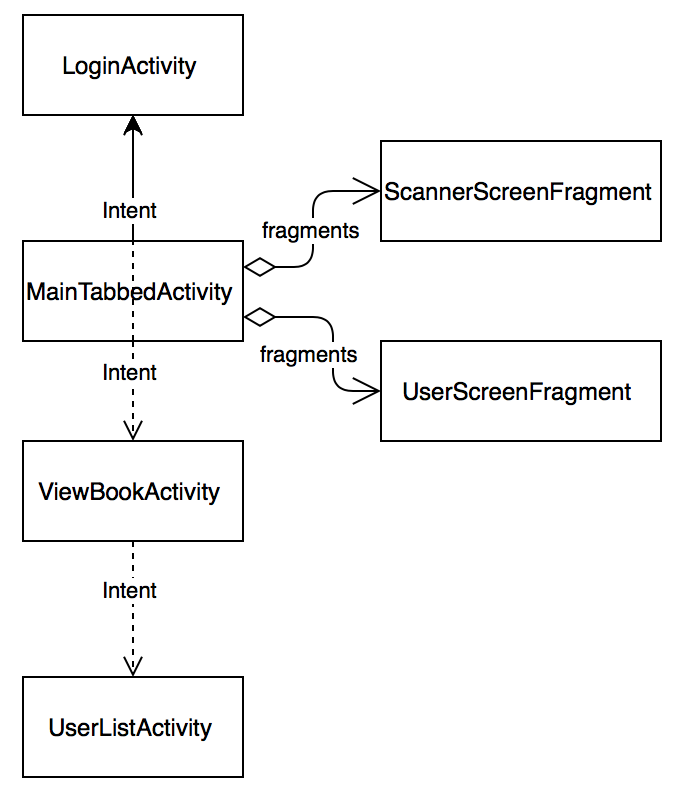
\includegraphics[height=7cm]{figs/v03/AndroidStructure-03.png}
\caption{Basic Android version 0.3 structure}
\label{fig:AndroidStructure03}
\end{figure}

    \item[Design] \hfill\\
There was not done any big changes with the design for this version, but most of the buttons, images and text were made bigger to follow the design standards. How it looked when the owner of a book looked at its information in version 0.3, is shown in Figure \ref{fig:book-view-v3}. More feedback of user actions was also added in this version, for instance showing a loading spinner when book information is loading.  

\begin{figure}
\centering
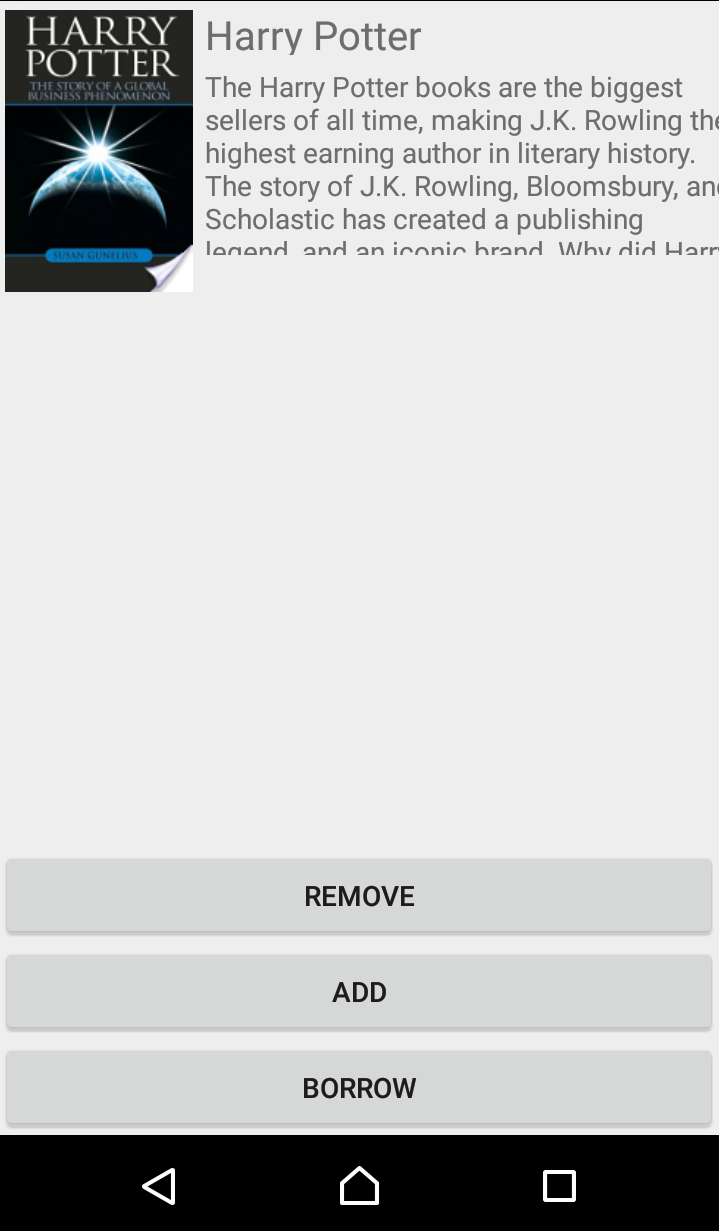
\includegraphics[height=7cm]{figs/v03/bookView03.png}
\caption{The activity showing book information in version 0.3 of the application}
\label{fig:book-view-v3}
\end{figure}

    \item[User feedback] \hfill\\
To get feedback on the new implemented features, more events where added to Mixpanel. Mixpanel now also allowed the application to track when a book was borrowed and when a book was returned. See table \ref{tab:mixpanel_table}.

    \item[Bug fixes] \hfill\\
After the version 0.2 of the application had been used, some errors were discovered. For instance, if a user scanned a barcode that could not be found in Google Books, the application crashed and displayed an error message. This was solved by handling the error from Google Books and displaying a message to the user that the book was not found. Another bug discovered in the last version was that the applications local realm database was deleted when the application closed, which meant that next time the application was launched the information stored in the database was no longer available. 
\end{description}

\subsubsection{iOS}
\begin{description}
    \item[Features] \hfill\\
The goal for this version for the iOS team was to make it possible to borrow books from other users, and return them. In order to borrow a book, the user had to scan the barcode, press the borrow button, and select the owner of the book form a list. As there were no way to filter owners at this point, all users who had the given book in their shelf would be displayed. When an owner was selected, a request would be sent to the \gls{backend} to update the information in the database.

Because borrowing books raised the need to identify individual users, a login feature had to be implemented. This was done by creating a new login view, and setting the user model representing the currently authenticated user as a class variable on the \code{User} class. Therefore, the local user would be accessible from all parts of the application. Which was beneficial when retrieving books, crowds and users related to the local user, from the server.

    \item[Design] \hfill\\
The overall design from version 0.2 was extended to include the new buttons necessary to borrow and return books. Some additional feedback was added to provide the user some information about the state of the application.

    \item[User feedback] \hfill\\
The integration of Mixpanel from version 0.2 was extended to also include reporting borrow and return events for books. This would allow the team to monitor how the new features were used.
\end{description}

\subsubsection{Backend}
The \gls{backend} seems mostly finished for books and book loans after the release of version 0.2, so the team just focused on bug fixes for those two areas. This means that there have not been that much real implementation for the \gls{backend} team this iteration. The team implemented a lot of \gls{ID}-validation, for instance that a user \gls{ID} that is added to a book as a loaner, actually is a user in the database.

For this version the \gls{backend} team researched APIs for getting information on norwegian books. The team also did a lot of research on the Docker software container framework, as the customer wanted us to wrap the whole \gls{backend} solution in it. \cite{docker} The team also looked more into deployment platforms, as the limitations of the free version of Heroku had become apparent. At this point the team were using the free level of service they offer, which is not much. \cite{heroku-pricing} It does not offer 24/7 uptime, which the team want for the server serving the stable API. The free level has to sleep 6 hours of every 24 hours. This means the service will be unreachable for a fourth of every 24 hours. 

To meet the demands the team looked after other options. The team talked to Microsoft about their Dreamspark-licenses (license for students) and what it gives access to on Microsoft Azure. \cite{microsoft-dreamspark} After talking with Microsoft on the phone, the team found that the DreamSpark-license does not cover running a server written in Node.

In addition the domain \url{http://crowdshelf.xyz} was bought, and \gls{PaaS}s like Digital Ocean was researched.\cite{digitalocean} The team decided to rent a so called ''droplet'', a virtual machine, from Digital Ocean. The domain was pointed at that virtual machine. Also see the preliminary studies, section \ref{prelim-digitalocean}, for more research on this \gls{PaaS}.


\subsection{Feedback}
From the feedback shown in table \ref{feedback-3} the team continued with the layout selected in the paper prototypes with focus on implementing clear feedback to the users when taking an action. 
\begin{table}[]
\centering
\begin{tabular}{|L{1.5cm}|L{1cm}|L{3cm}|L{7cm}|}
\hline
\textbf{Gender} & \textbf{Age} & \textbf{Occupation} & \textbf{Problems/ comments} \\
\hline
Male & 20-30 & Student & Completed all the tasks without ant problemts. Would like to confirm when returning a book. \\
\hline
Female & 20-30 & Student & Completed the tasks, but did not find the “done”-button immediately. Would also like an explanation of the buttons first time the app is used. \\
\hline
Male & 20-30 & Student & Completed the tasks without difficulty, but would like an explanation of the buttons in Viewbook, specially remove vs return. \\
\hline
Female & 20-30 & Student & Did not understand the scanner, and had difficulties with the concept of the application. \\
\hline
\end{tabular}
\caption{Feedback regarding the usability test of the paper prototype of version 0.3}
\label{feedback-3}
\end{table}
Regarding feedback from the use of the application the team has obtained some new users, but still not enough to make the numbers applicable for analysis to learn from. 

Although there still is a question of how many users can be obtained to collect user data from the application, the analysis done from questions and usability test gave some answers to the assumption of this version. The answer to the question about whether the users are borrowing books is twofold. The same is the case for the answer about if they are having trouble keeping track of where those books are.

At this stage the applications main user base is students and companies, and the book habits are quite different in those two areas. The students tend to borrow books about twice a year (each semester), while the employees at Netlight often borrow books from the company. In both cases people have some trouble keeping track of the books, but this problem is somewhat more relevant amongst the students. 

As a result of these results the team decided to focus on the company needs of the application. The students are still welcome to use the application, but because they borrow books so rarely there will not be enough use of the application to get some real data from their use. 


\subsection{Version progress}

In this version the progression has continued in a stable manner with tasks being completed within their due date. At the end of the version, as shown in figure \ref{fig:progress-3}, four of the team members had a big delivery in another course, so the progress want a little slow those days. However in an overall manner the progression of the project has stabilized, much because the team members have achieved a deeper understanding of the technologies they are working with, and also the concepts and ideas behind the Lean Startup.

Observed in appendix \ref{app:release-note-3}, the release note of version 0.3, almost all the tasks completed are related to the user stories selected for the version. This is due to the focus of the version of having clear goals and trying to do what has to be done to complete the version instead of fixing other problems. Of course there are tasks that has to be completed not related to the stories, but the team worked towards a common goal that they all felt they had decided together. 

The blog posts to keep information flow to the customer and supervisor are shown in figure \ref{fig:week-six} and \ref{fig:week-seven}. These explain what is performed by the team the weeks of the iteration that is version 0.3, both technical and non-technical.



\begin{figure}
\centering
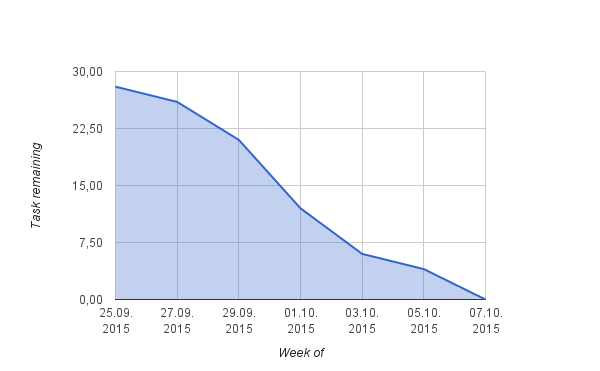
\includegraphics[height=10cm]{figs/v03/progress3.png}
\caption{Task progress version 0.3}
\label{fig:progress-3}
\end{figure}

\begin{figure}
\centering
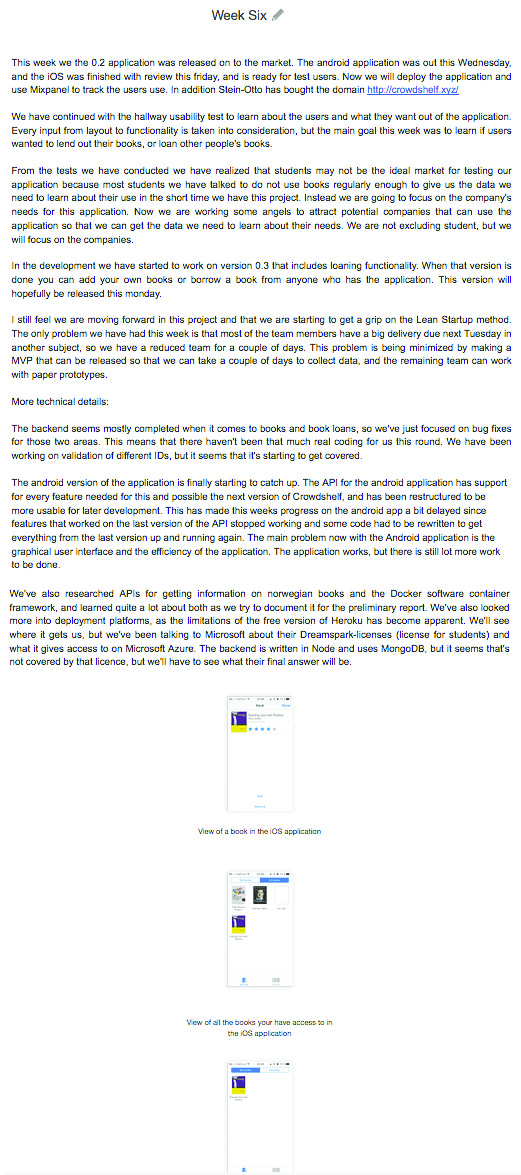
\includegraphics[height=22cm]{figs/v03/WeekSix.jpg}
\caption{Blog post from week 40}
\label{fig:week-six}
\end{figure}

\begin{figure}
\centering
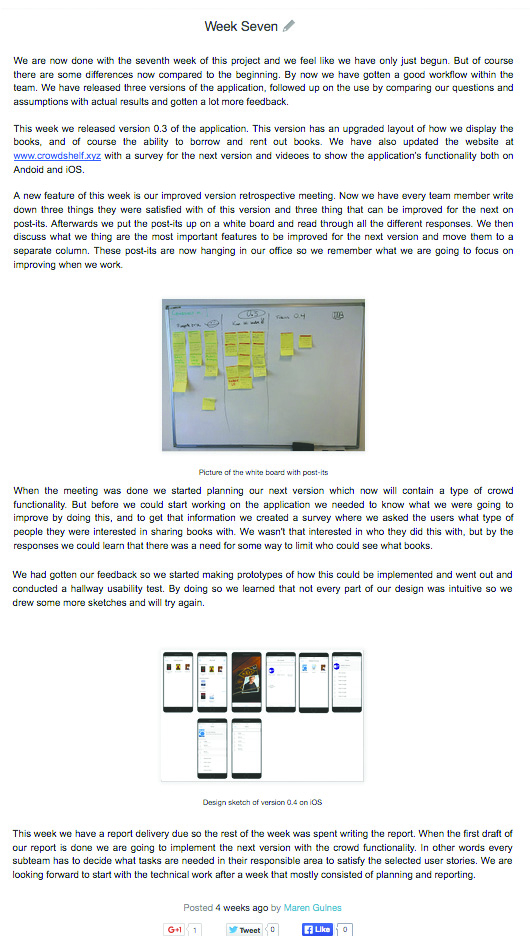
\includegraphics[height=22cm]{figs/v03/WeekSeven.jpg}
\caption{Blog post from week 41}
\label{fig:week-seven}
\end{figure}

\subsection{Review and retrospective}
During this version the team decided, together with the customer representative, to focus on the company parts of the application, and to satisfy those needs. In discussion with him the team came up with some potential businesses that had mentioned their interest in the application. The interests were a primary school in Oslo and the police attorneys at Grønland police station.

Minutes from the costumer meeting is located in appendix \ref{app:customer-minutes-6} and \ref{app:customer-minutes-7}.

As a consequence of the possible new interests a new feature was discussed, namely the development a custom book information provider. The teams \gls{backend} lead research to see if he could find any norwegian book information provider that could satisfy the need to those potential new businesses, but ended up concluding there was no such API. With that as basis the idea of a new system to support this came to life. 

When version 0.3 of the application was released the team had a retrospective meeting. As of this version that meeting was performed in a different manner than the previous retrospective meetings. From a suggestion from the customer representative, the meeting was now performed using post-it notes and whiteboard. Every team member wrote down three things they thought went well during the version, and three points they thought could be improved. Out of those points, two were selected to be the main focus in the next version. 

As illustrated in the picture of the whiteboard found in figure \ref{fig:retrospective-3} the “Went well” column and “Can be improved” have approximately the same amount of notes. A goal of the project is to shorten down the “Can be improved column”. The positive aspects of this version are focused around the improvements in development and the communication within the team, and between sub-teams. The improvement points were mainly about getting a better structure within the Android team, and to continue to work on upholding the version control and JIRA delegation. 

The focus points from version 0.3 were the delegation of tasks within the Android team, and improving the connection between the iteration results and the assumption selected in the version. To improve the task delegation in the Android team, the Android lead should focus on creating tasks to the selected user stories and delegate them to the other team members. To improve the coupling between assumption and results the assumption will be written down for each iteration, and each result will be measured with thought to the assumption.

\begin{figure}
\centering
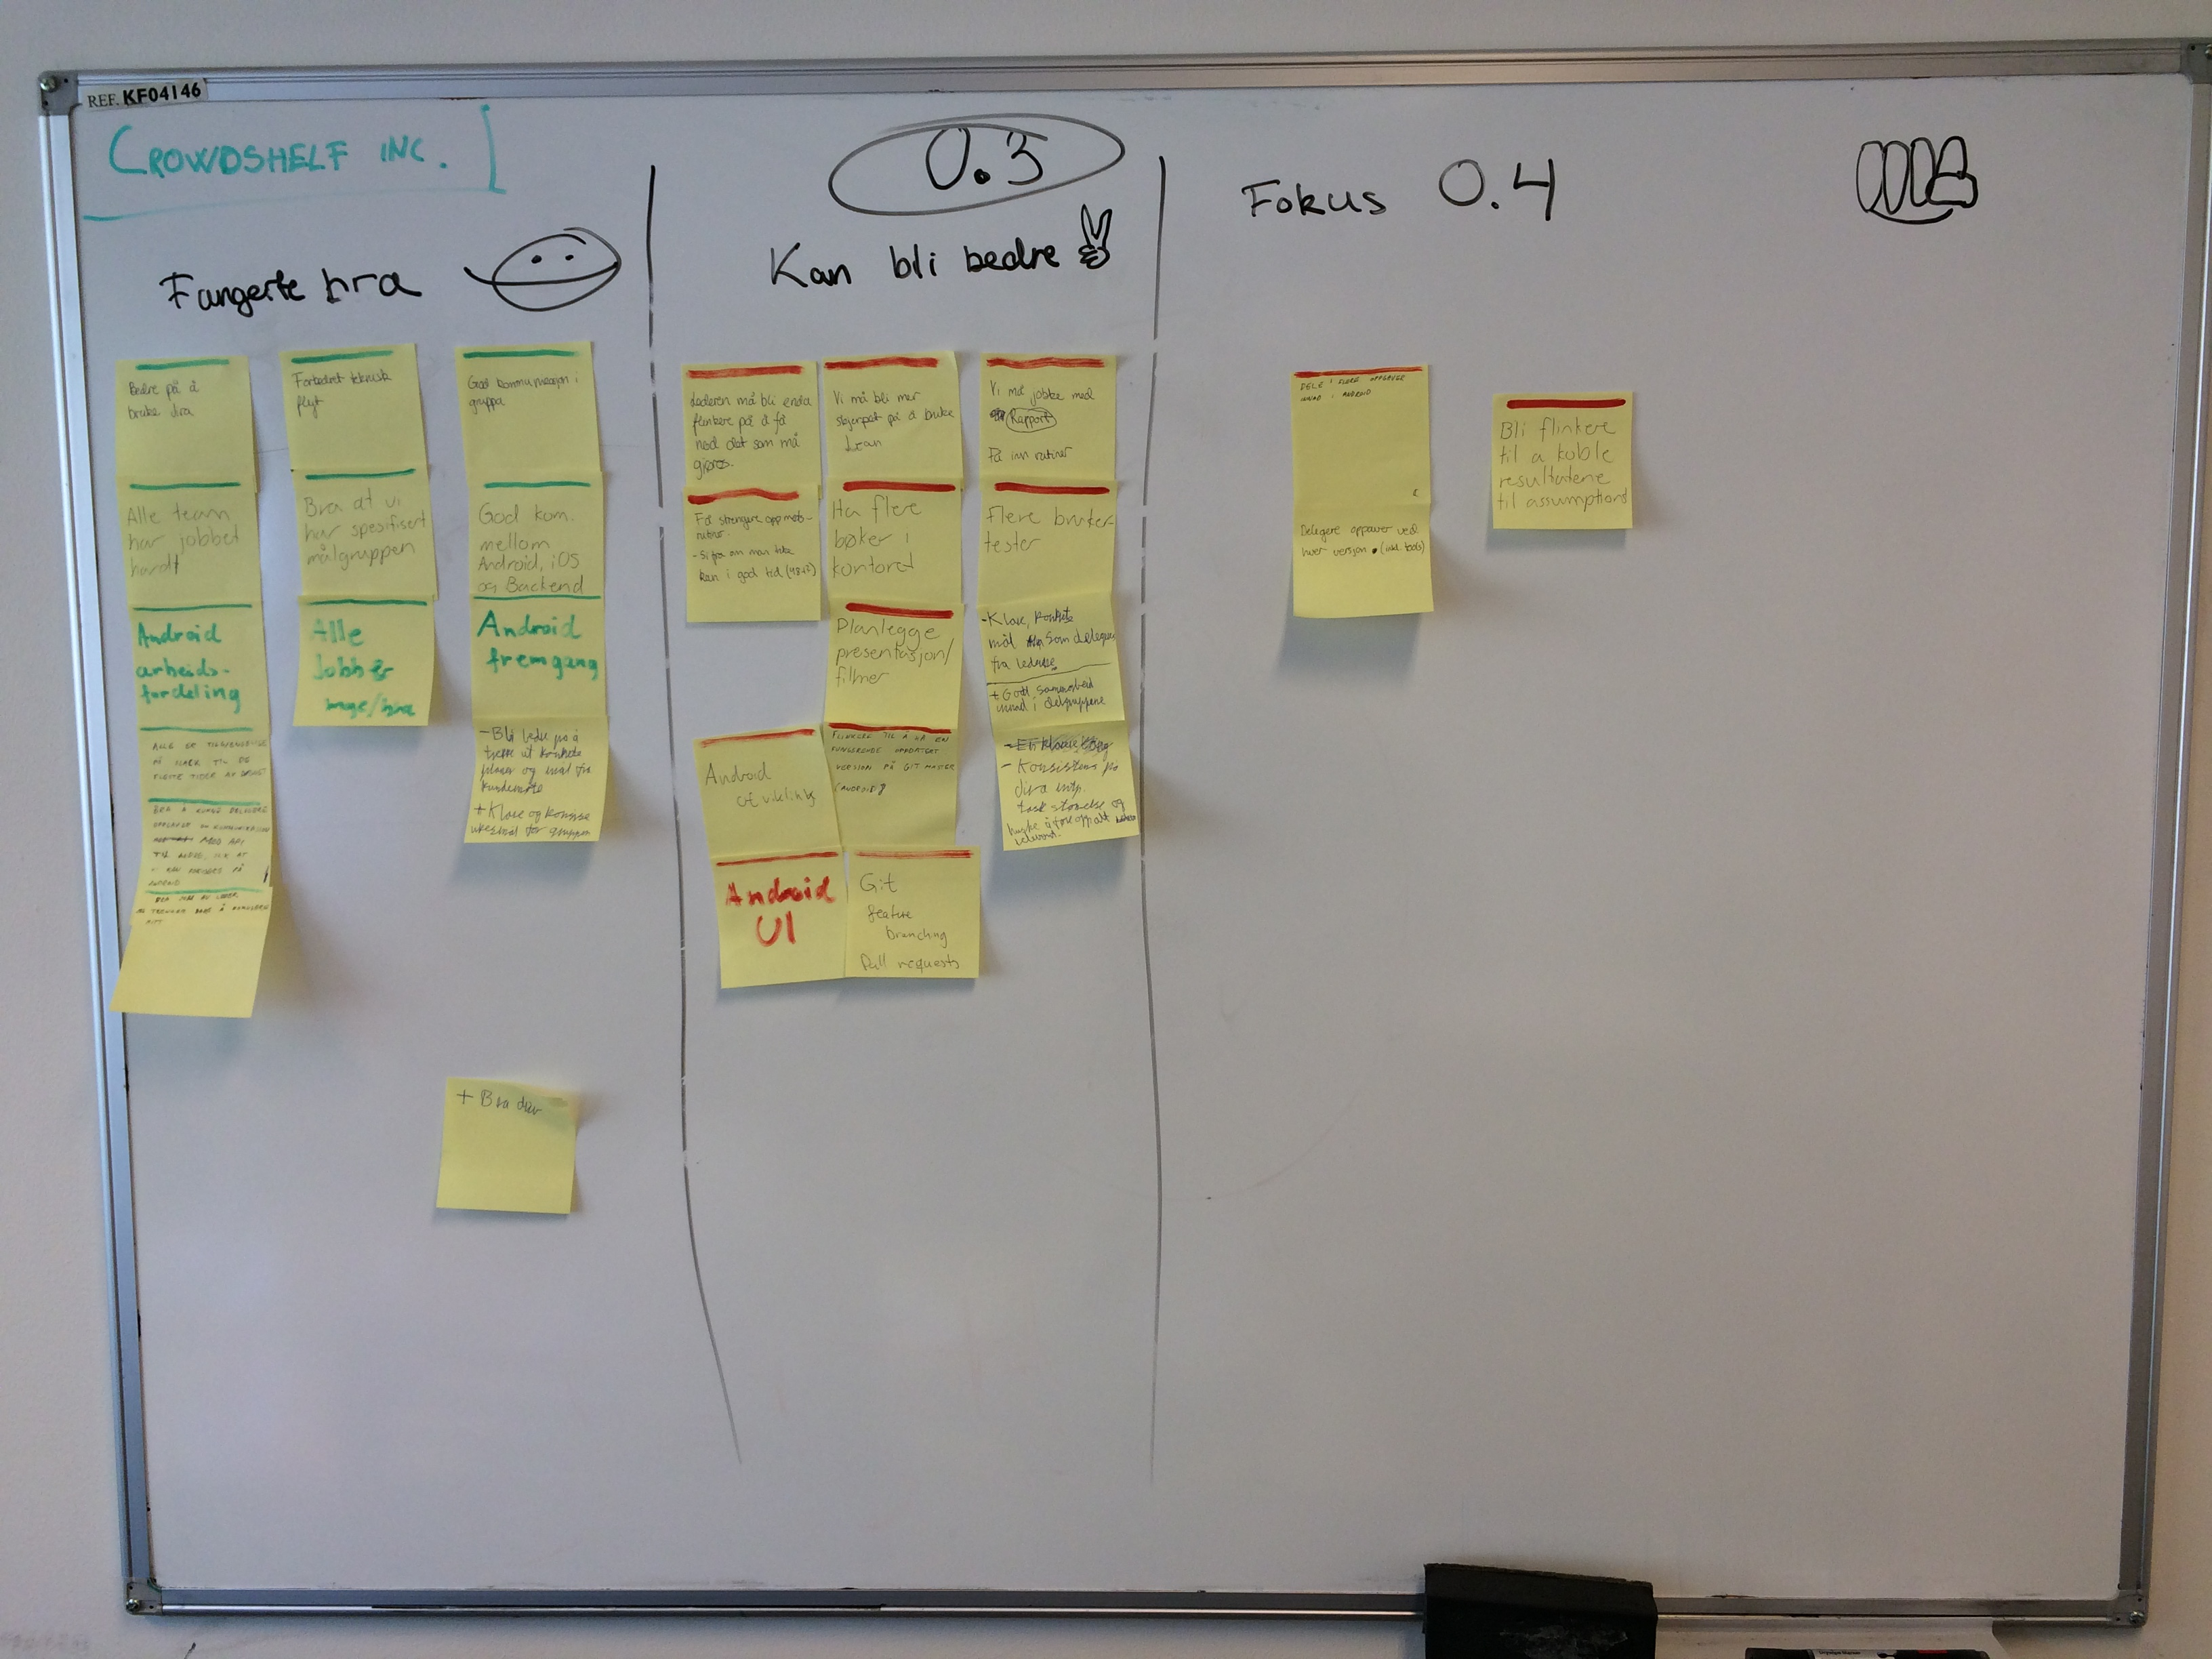
\includegraphics[height=10cm]{figs/v03/retrospective-3.JPG}
\caption{Picture of the whiteboard from retrospective meeting of version 0.3}
\label{fig:retrospective-3}
\end{figure}

\subsection{Summary}
At the beginning of version 0.3 the assumption was that the users borrow books and from time to time have trouble keeping track of where those books are in the sense of who the user have borrowed the book from or to. What was learned during this version was that the student users do not borrow book often enough to be a priority user in this project. Businesses on the other hand have a lot of books that people can borrow on a daily basis. 

As a consequence of the results the team has decided in agreement with the customer to focus on the business needs in the application. One of those needs is a possible book service where the users can add their own books if it does not exist in the Google Books database. The team will also focus on learning about the real business needs in association with the application in the next version by sending out a survey asking about their book habits. Until now their book habits are only gotten by asking unofficially and are therefore only indications.

The change in the performance of the retrospective meeting made it easier to get all the team members opinions and gave the team a constant visual, as the notes always were up on the board of what they had agreed to focus on.   
